\documentclass[tikz,border=8pt]{standalone}
\usepackage[T1]{fontenc}\usepackage{lmodern}\usepackage{pgfplots}\pgfplotsset{compat=1.18}
\begin{document}
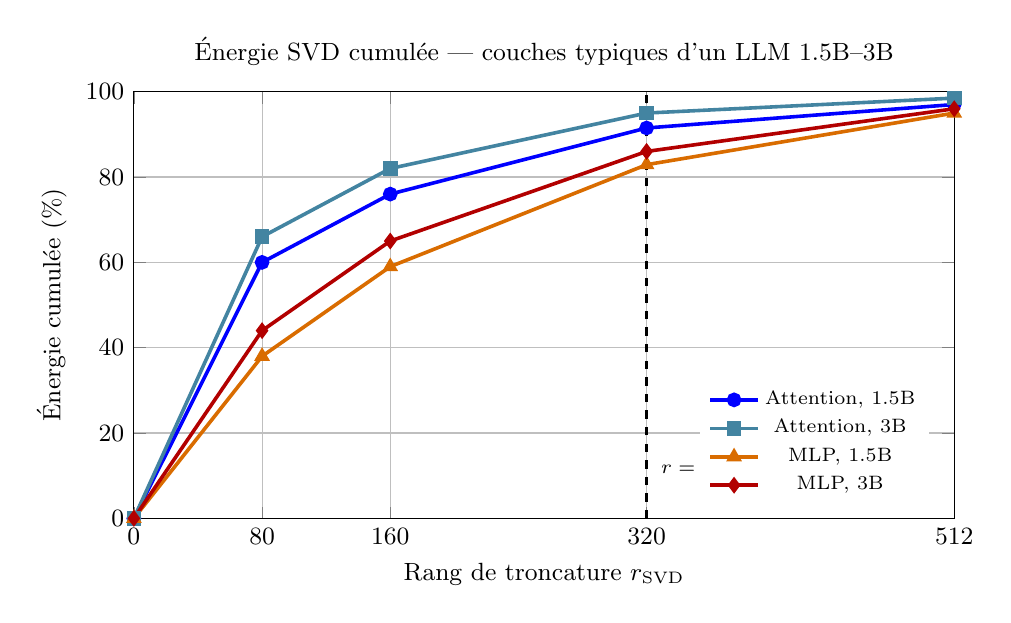
\begin{tikzpicture}
\begin{axis}[width=12cm,height=7cm,font=\small, title={Énergie SVD cumulée — couches typiques d'un LLM 1.5B–3B}, xlabel={Rang de troncature $r_{\mathrm{SVD}}$},ylabel={Énergie cumulée (\%)},xmin=0,xmax=512,ymin=0,ymax=100,xtick={0,80,160,320,512},ytick={0,20,40,60,80,100},grid=major,legend pos=south east,legend style={font=\scriptsize,fill=white,draw=none},every axis plot/.append style={line width=1.3pt}]
% Reconstructed schematic curves; 82.9% and 91.5% are called out at r=320 in the source.
\addplot[blue,mark=*] coordinates {(0,0)(80,60)(160,76)(320,91.5)(512,97)};\addlegendentry{Attention, 1.5B}
\addplot[cyan!60!black,mark=square*] coordinates {(0,0)(80,66)(160,82)(320,95)(512,98.5)};\addlegendentry{Attention, 3B}
\addplot[orange!85!black,mark=triangle*] coordinates {(0,0)(80,38)(160,59)(320,82.9)(512,95)};\addlegendentry{MLP, 1.5B}
\addplot[red!70!black,mark=diamond*] coordinates {(0,0)(80,44)(160,65)(320,86)(512,96)};\addlegendentry{MLP, 3B}
\addplot[dashed,black] coordinates {(320,0)(320,100)};\node[anchor=south west,font=\scriptsize] at (axis cs:323,7) {$r=320$ (papier)};
\end{axis}\end{tikzpicture}
\end{document}
